\documentclass[12pt, a4paper, oneside]{article}
\usepackage[left=1in, right=1in]{geometry}
\usepackage[utf8]{inputenc}
\usepackage[T1]{fontenc}
\usepackage{polski}
\usepackage{graphicx}
\usepackage{listings}
\usepackage{cite}
%\usepackage[numbers,sort&compress]{natbib}
\usepackage{notoccite}
\usepackage{multirow}
\usepackage{float}



\usepackage{mathtools, amsthm, amssymb}
\mathtoolsset{showonlyrefs, mathic}

\newtheorem{theorem}{Twierdzenie}
\newtheorem{lemat}{Lemat}
\newtheorem{uwaga}{Uwaga}
\newtheorem{przyklad}{Przykład}
\newtheorem{wniosek}{Wniosek}

\newcommand{\mychapter}[2]{
	\setcounter{chapter}{#1}
	\setcounter{section}{0}
	\chapter*{#2}
	\addcontentsline{toc}{chapter}{#2}
}


\author{Paweł Budzyński \\ Wydział Matematyki, Politechnika Wrocławska}
\title{\textbf{Wykorzystanie sieci neuronowych w problemie wykrywania uszkodzeń lokalnych w maszynach górniczych}}
\date{2018 \\ Październik}

\begin{document}
	\maketitle
	%\tableofcontents
	%\mychapter{1}{Wstęp}
	\newpage
	\section{Wstęp}
	Tematem pracy jest wykorzystanie sieci neuronowych w problemie wykrywania uszkodzeń lokalnych w maszynach górniczych. Zadanie polega na przetworzeniu sygnału diagnostycznego oraz dokonaniu na jego podstawie decyzji o możliwości wystąpienia uszkodzenia w mechanizmach maszyny górniczej.
	{\Huge zdjeica maszyny i jakis czujnikow}
	
	\subsection{Opis problemu}
	
	Uszkodzenia lokalne są uszkodzeniami występującymi w łożyskach i przekładniach maszyn górniczych. Ich powstawanie uzależnione jest od zmiennych warunków eksploatacyjnych. Uszkodzenie w początkowym stanie obniża sprawność maszyny a ostatecznie może doprowadzić do jej unieruchomienia. Jest to szczególnie problematyczne ponieważ kopalnia dysponuje często jedną lub dwiema takimi maszynami, dodatkowo każda z nich pracuje wyłącznie na swoim stanowisku, nie są one przemieszczane. Detekcja uszkodzenia we wstępnym stadium rozwoju jest ważnym zagadnieniem ponieważ pozwala z wyprzedzeniem określić moment konserwacji urządzenia. 
	
		W detekcji uszkodzeń najczęściej wykorzystuje się diagnostykę wibroakustyczną. Metoda polega na umieszczeniu sensora na obudowie urządzenia, następnie następuje pomiar drgań. Otrzymany sygnał zawiera pewien zakres informacji na podstawie których możemy wnioskować o zaistnieniu uszkodzenia w urządzeniu. W przypadku opisywanych uszkodzeń okazuje się że ich obecność objawia się poprzez cykliczne impulsy w sygnale.
	% Sygnał z pulsacjami i bez pulsacji
	{\LARGE tutaj zdjecia maszyny i sygnaly z impulsami widocznymi, niewidocznymi}
	
	Jednak w zależności od stopnia uszkodzenia pulsacje mogą mieć różne amplitudy, w przypadku wczesnego stadium rozwoju uszkodzenia najczęściej nie wystają one ponad poziom szumu.
	Można zatem stwierdzić że detekcja uszkodzenia, z punktu widzenia matematyki, sprowadza się do wykrycia cyklicznych impulsów. 
	
	%wykrywanie uszkodzeń lokalnych jest jednym z \cite{Zimroz01}
	%Uszkodzenia lokalne powstające w przekładniach kół czerpakowych maszyn górniczych, są to na %przykład ubytki, pęknięcia, wykruszone zęby.  Najskutecznejszą obecnie metodą pozyskania sygnału %jest diagnostyka wibroakustyczna, okazuje się że uszkodzenia takie objawiają się cyklicznymi %pulsacjami w sygnale. Amplituda pulsacji zależy od stopnia uszkodzenia. Z punktu widzenia %matematyki detekcja takiego uszkodzenia polega na wykryciu, zazwyczaj niewidocznych na pierwszy %rzut oka, pulsacji w sygnale diagnostycznym. 
	
	\subsection{State of the art}
	prztumaczyc dokument ze strony wylomanskiej 
	{\Huge tutaj jakies odleglosci od rozkladu normalnego, spektrogramy itd}
	
	
	\subsection{Sieci neuronowe}
	Sieci neuronowe można zdefiniować jako struktury matematyczne realizujące obliczenia lub przetwarzające sygnały poprzez rzędy elementów zwanych sztucznymi neuronami.
	Sieci neuronowe są jedną z prężnie rozwijających się technologii nauczania maszynowego i szeroko wykorzystywane w pracach nad sztuczną inteligencją.
	Prężny rozwój dziedziny zapoczątkowało wynalezienie sztucznego perceptronu w 1957r. Był to model sztucznego neuronu pozwalającego na binarną klasyfikację liniowo separowalnych danych. Wraz z upływem czasu pojawiają się kolejne modele neuronów i rodzaje sieci neuronowych. 
	\\
	Chociaż jest to stosunkowo nowa technologia, znalazła już ona szereg zastosowań w wielu dziedzinach. Do najpopularniejszych zastosowań należy przetwarzanie obrazu takie jak rozpoznawanie twarzy, detekcja obiektów, wykrywanie zmian nowotworowych \cite{nnnature}, przetwarzanie mowy \cite{nnspeech} czy też autokorekta i podpowiadanie słów w klawiaturach smartfonów \cite{nngboard}.
	
	\newpage
	
	
	%\chapter{Metodologia}
	\section{Metodologia}
	Zakres wykonanej pracy obejmuje poszukiwanie optymalnego rozwiązania dla postawionego problemu. Na ten problem składają się wybór i przygotowanie danych uczących model oraz zaprojektowanie skutecznego modelu. 
	W kolejnych krokach opisano narzędzia i techniki wykorzystane w tym celu. Ponieważ sieci neuronowe wymagają znaczącej ilości danych, a ich zdobycie w przypadku zaawansowanych maszyn górniczych jest problematyczne, pracę należało zacząć od stworzenia sytemu symulowania sygnałów o zbliżonych cechach oraz wygenerowania zbioru danych (\textit{ang. dataset}). Następnie poruszony zostanie temat tak zwanej ekstrakcji cech, wstępnej obróbki danych w celu stworzenia najlepiej opisujących je cech. Finalnie możliwe jest przystąpienie do projektowania, trenowania i testowania sieci w celu stworzenia możliwie skutecznego modelu.
	\subsection{Symulowanie zbioru danych uczących} 
	
	\subsection{Wstępne przetwarzanie danych}
	Przed przystąpieniem do uczenia sieci neuronowej niezbędne jest przygotowanie zestawu danych uczących. W dalszej pracy przetestowano dwa podejścia, jedno z użyciem surowego sygnału, drugie polegające na przygotowaniu statystyk opisujących sygnał. Zadanie polega na wykryciu pulsacji w sygnale diagnostycznym dlatego wybór statystyk opisujących sygnał musi odpowiadać postawionemu zadaniu. Dla opisania zmienności sygnału posłużą następujące estymatory:
	\begin{itemize}
		\item Wartość maksymalna
		\item Wartość minimalna
		\item Wariancja
		\begin{equation}
			Var (X) = \frac{1}{n-1} \sum_{i=0}^{n} \left(x_{i} - \mu\right)^{2}
		\end{equation}
		\item Kurtoza
		\begin{equation}
			Kurt (X) = \frac{\frac{1}{n} \sum_{i=0}^{n}\left(x_{i} - \mu\right)^{4}}{\sigma^{4}} - 3
		\end{equation}
		\item Skośność
		\begin{equation}
			Skew (X) = 3 \frac{\mu - m}{\sigma}
		\end{equation}
	\end{itemize}

	
	
	\subsection{Zastosowanie sieci neuronowych}
	Sieci neuronowe są strukturami realizującymi przetwarzanie danych poprzez rzędy elementów. Siecią użytą w pracy jest tak zwany perceptron wielowarstwowy. Jego bazowym elementem jest perceptron zaprezentowany poniżej. Składa się on z wejść wraz z wagami, funkcją sumującą oraz funkcją aktywacji. W przypadku użycia funkcji kroku perceptron pozwala na binarną klasyfikację liniowo separowalnych danych. 
	\begin{figure}[H]
		\centering
		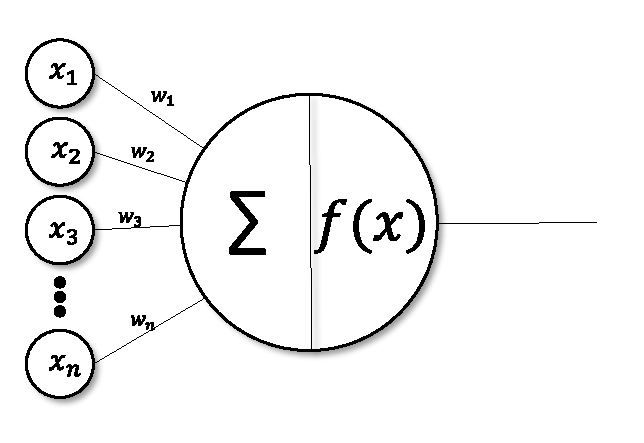
\includegraphics[width=10cm]{images/perceptron_c.pdf}
		\caption{Perceptron}
	\end{figure}
	W trakcie dalszych badań odkryto że połączenie wielu perceptronów pozwala na stworzenie struktury skutecznej nie tylko dla liniowo separowalnych danych. Tak powstał perceptron wielowarstwowy, popularna sieć neuronowa skuteczna w wielu zastosowaniach. Wyzwaniem jest wyznaczenie wag dla poszczególnych wejść. Najczęściej to zadanie jest realizowane poprzez algorytm wstecznej propagacji polegający na obliczaniu błędu na wyjściu z sieci a następnie przekazywaniu go wstecz tak aby poszczególne warstwy mogły zmodyfikować swoje wagi. 
	\begin{figure}[H]
		\centering
		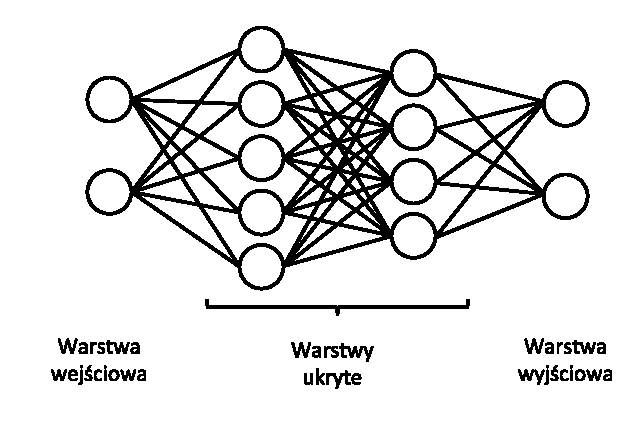
\includegraphics[width=10cm]{images/siec_c.pdf}
		\caption{Perceptron wielowarstwowy}
	\end{figure}
	
	Testowanie skuteczności sieci odbywać się będzie przy pomocy techniki nazywanej walidacją krzyżową. Polega ona na podziale całości danych na części a następnie wybierane kolejno jednej z nich jako zbioru testowego, używając reszty danych do nauczenia sieci. Zbierając wyniki dla wykonanych prób możliwe jest określenie jakości rozwiązania. 
	\begin{figure}[H]
		\centering
		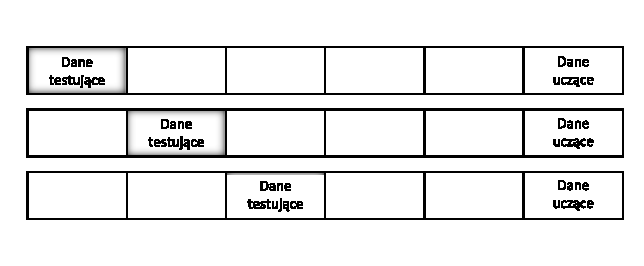
\includegraphics[width=10cm]{images/walidacja_c.pdf}
		\caption{Walidacja krzyżowa}
	\end{figure}

	\subsection{Trening sieci neuronowej}
	tutaj schemat kompletnego działąnia z podsumowaniem tego co bylo wczesniej i opisem jak dziala
	\begin{figure}[H]
		\centering
		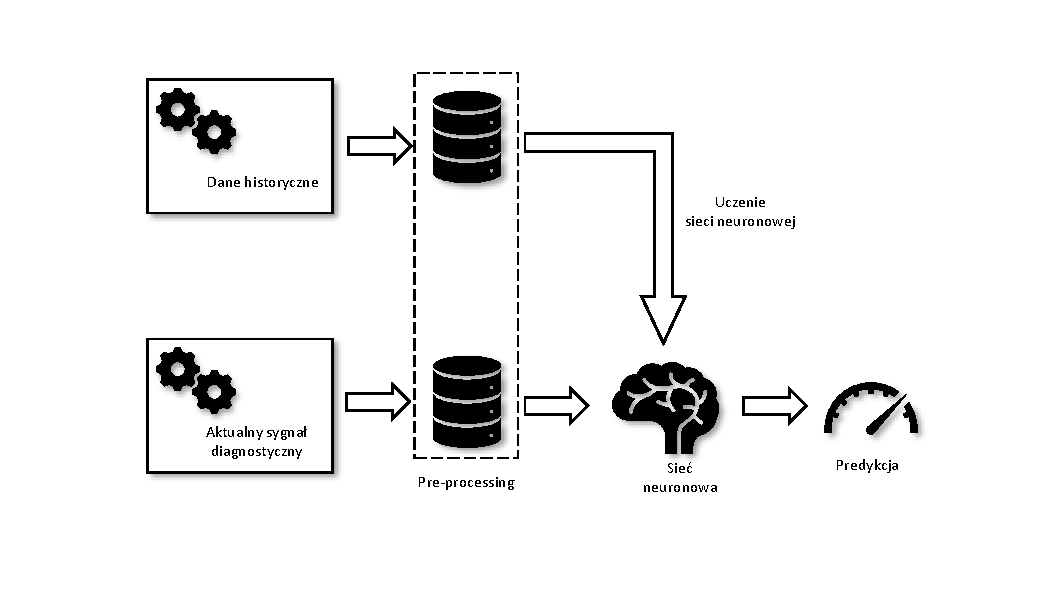
\includegraphics[width=16cm]{images/total_proc.pdf}
		\caption{Schemat przebiegu pracy systemu wykrywania uszkodzenia}
	\end{figure}
	\subsection{System klasyfikacji uszkodzeń}
	Finalnym zadaniem jest stworzenie całości systemu monitorującego który dokonywałby predykcji na postawie wprowadzonego sygnału. 
	\begin{figure}[H]
		\centering
		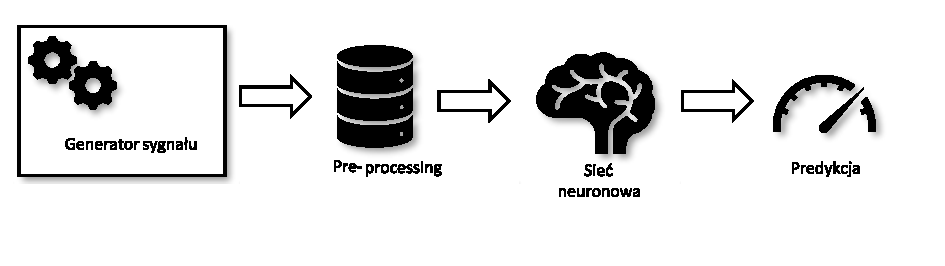
\includegraphics[width=14cm]{images/workflow_c.pdf}
		\caption{Schemat przebiegu pracy systemu wykrywania uszkodzenia}
	\end{figure}

	W dalszych rozdziałach opisany zostanie proces wykorzystania powyższych metod w celu opracowania optymalnego rozwiązania. Rozpoczynając od określenia metodyki projektowania i testowania sieci neuronowej poprzez trening i wybór najlepszego modelu. Ostatecznie zaprezentowane zostanie przykładowe zastosowanie opracowanego modelu w teoretycznym systemie monitorującym pracę maszyny górniczej. 
	
	
	
	% opis dzialania sieci neuronowej jak sadze
	
	
	
	
	
	\newpage
	
	%\chapter{Wyniki dla danych symulowanych}
	\section{Projektowanie sieci neuronowej}
	Skuteczność rozwiązania silnie zależy od użytej sieci. Projektowanie sieci polega na doborze tak zwanych hiperparametrów (\textit{ang. hyperparameters}). Zalicza się do nich między innymi:
	\begin{itemize}
		\item Liczba warstw ukrytych
		\item Liczba neuronów w warstwach
		\item Algorytm nauczania oraz jego parametry
		\item Funkcje aktywacji w neuronach.
	\end{itemize}

	Nie istnieje skuteczna metoda doboru parametrów, przy zastosowaniu złożonych sieci badacze najczęściej polegają na swoim doświadczeniu oraz intuicji. Na potrzeby tego zadania przeprowadzono szereg eksperymentów mających na celu określić najskuteczniejszą sieć do wykonania postawionego zadania. \\
	
	Żeby tego dokonać należy ustalić sposób pomiaru skuteczności danej sieci, w tym celu posłużono się macierzą pomyłek oraz zdefiniowanymi przy jej pomocy miarami.

	\begin{table}[H]
		\begin{tabular}{lccc}
			& \multicolumn{1}{l}{}                    & \multicolumn{2}{c}{\textbf{klasa rzeczywista}}                                                                                                                                      \\ \cline{3-4} 
			& \multicolumn{1}{c|}{}                   & \multicolumn{1}{c|}{\textbf{pozytywna}}                                                  & \multicolumn{1}{c|}{\textbf{negatywna}}                                                  \\ \cline{2-4} 
			\multicolumn{1}{c|}{\multirow{2}{*}{\textbf{klasa predykowana}}} & \multicolumn{1}{c|}{\textbf{pozytywna}} & \multicolumn{1}{c|}{\begin{tabular}[c]{@{}c@{}}prawdziwie\\ pozytywna (TP)\end{tabular}} & \multicolumn{1}{c|}{\begin{tabular}[c]{@{}c@{}}fałszywie\\ pozytywna (FP)\end{tabular}}  \\ \cline{2-4} 
			\multicolumn{1}{c|}{}                                            & \multicolumn{1}{c|}{\textbf{negatywna}} & \multicolumn{1}{c|}{\begin{tabular}[c]{@{}c@{}}fałszywie\\ negatywna (FN)\end{tabular}}  & \multicolumn{1}{c|}{\begin{tabular}[c]{@{}c@{}}prawdziwie\\ negatywna (TN)\end{tabular}} \\ \cline{2-4} 
		\end{tabular}
	\caption{Macierz pomyłek}
	\end{table}

	\begin{center}
		\begin{enumerate}
			\item Dokładność (\textit{ang. accuracy})
			\begin{equation}
				acc = \frac{TP + TN}{P + N}
			\end{equation}
			\item Czułość (\textit{ang. recall}) - odsetek prawdziwie pozytywnych
			\begin{equation}
				recall = \frac{TP}{TP + FN}
			\end{equation}
			\item Precyzja (\textit{ang. precision})
			\begin{equation}
				precision = \frac{TP}{TP + FP}
			\end{equation}
			\item F1 - średnia harmoniczna precyzji i czułości 
			\begin{equation}
				F1 = 2 \cdot \frac{precision \cdot recall}{precision + recall}
			\end{equation}
		\end{enumerate}
		
	\end{center}
	
	Badanie skuteczności sieci opiera się na metodyce walidacji krzyżowej czyli podziału zbioru danych na części a następnie użycie każdej z kolejno do testowania, reszta do uczenia <- to do metodyki
	

	\subsection{Zależność od danych wejściowych}
	Pierwszy eksperyment będzie postawą do decyzji o tym jakich danych należy użyć do uczenia sieci. Należy porównać jak uczy się sieć w zależności od danych wejściowych. Porównane zostaną dwa podejścia: użycie surowego sygnału oraz wstępnie przetworzonego. 
	
	\begin{enumerate}
		\item Surowy sygnał podeście pierwsze
			\subitem dane wejściowe: 4096
			\subitem warstwy ukryte: 1000 - 500 - 200
			\subitem liczba wag: 
		
		\item Surowy sygnał podejście drugie
			\subitem dane wejściowe: 4096
			\subitem warstwy ukryte: 500 - 200
			\subitem liczba wag:
			
		\item Estymatory sygnału
			\subitem dane wejściowe: 8
			\subitem warstwy ukryte: 5 - 3 - 2
			\subitem liczba wag: mało
	\end{enumerate}
	
	Wyniki eksperymentu prezentują sie następująco.
	

	\begin{figure}[H]
		\centering
		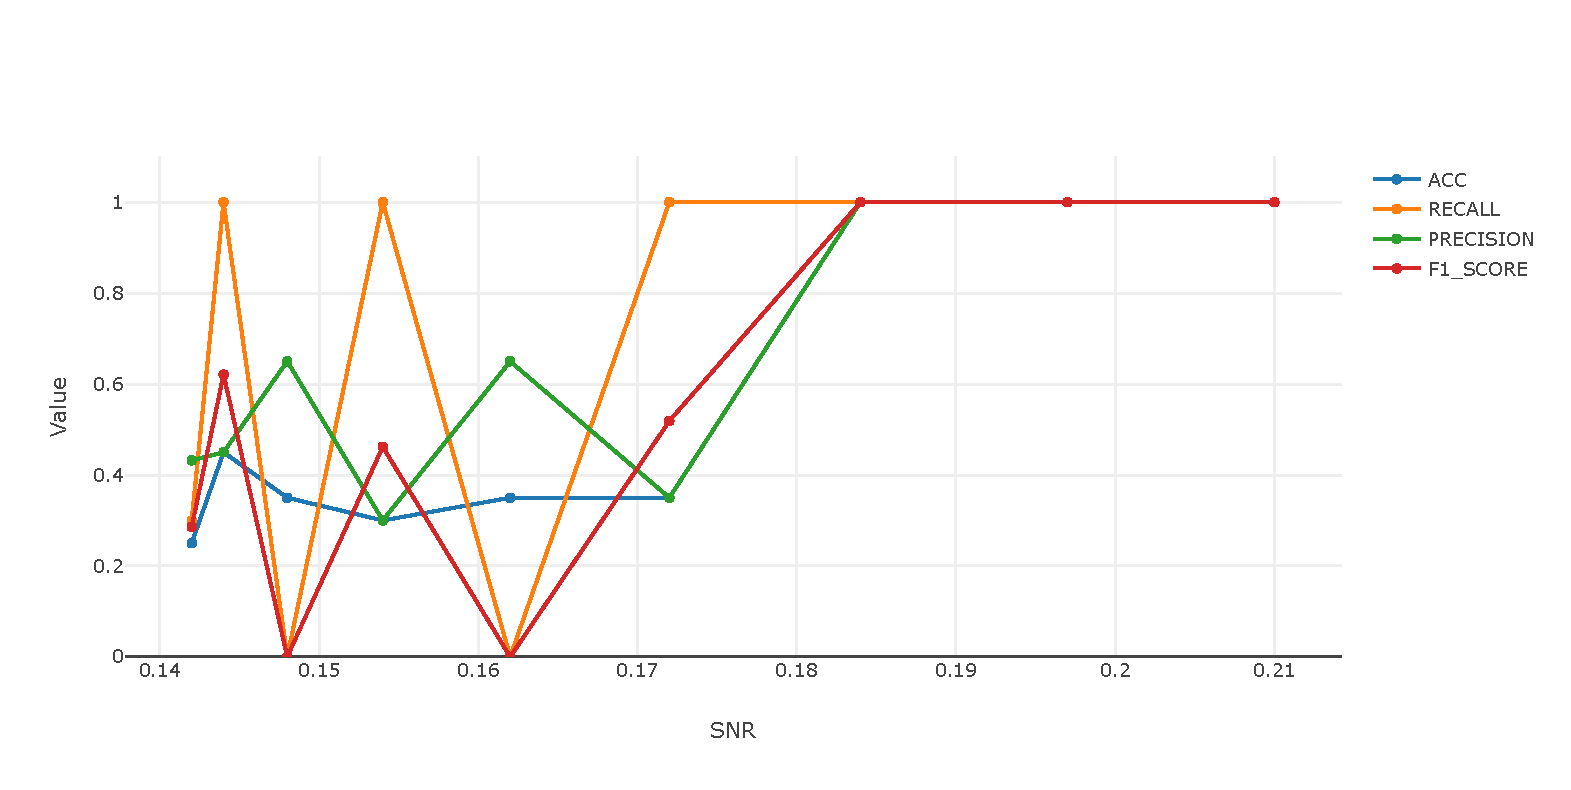
\includegraphics[width=14cm]{images/nn_full_1000_500_200.pdf}
		\caption{Wyniki surowego sygnału, architektura -1000-500-200-}
	\end{figure}

	\begin{figure}[H]
		\centering
		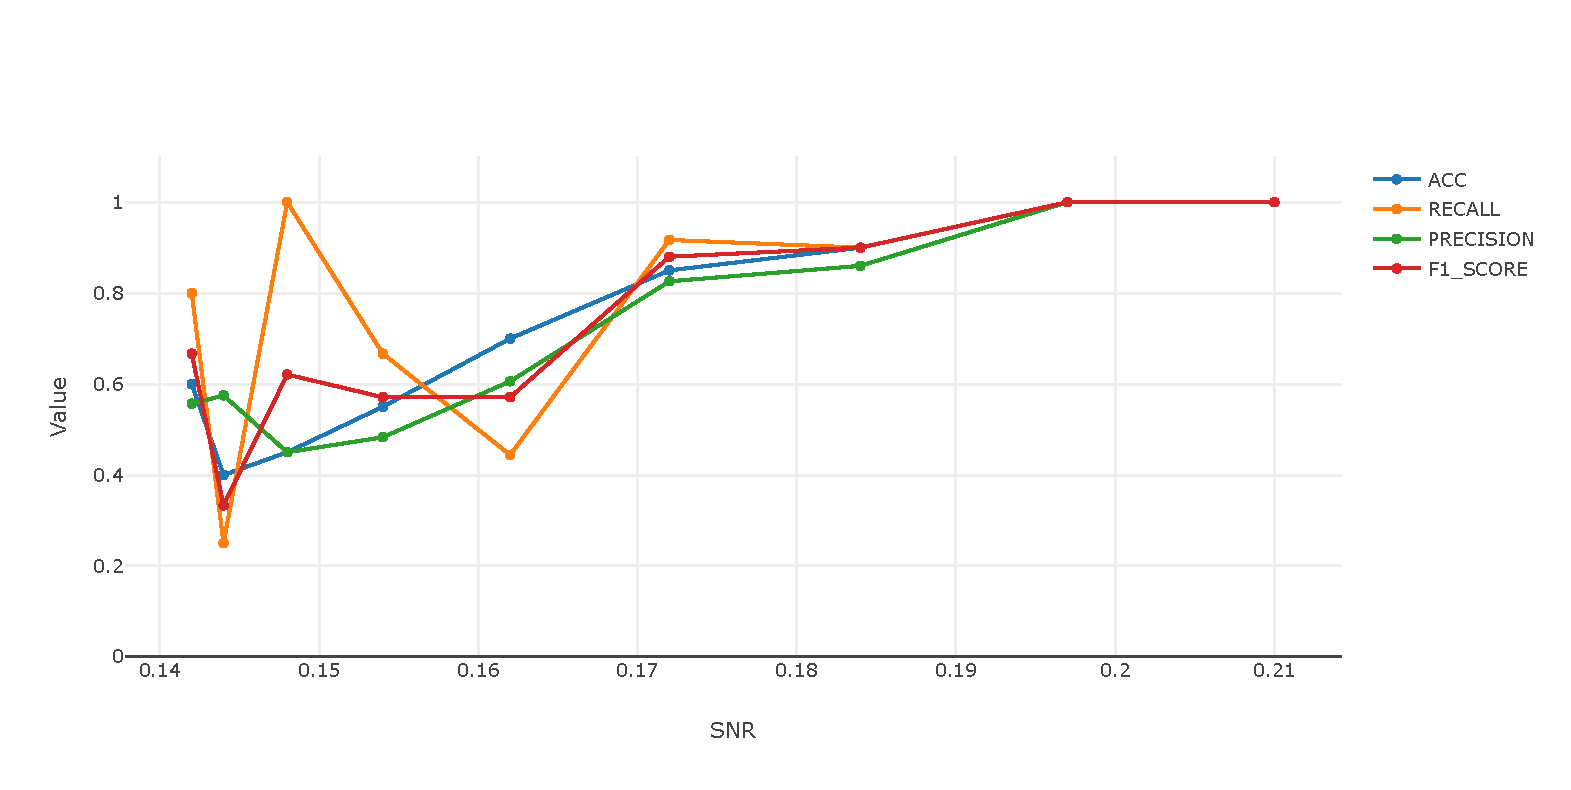
\includegraphics[width=14cm]{images/nn_full_signal_500_200.pdf}
		\caption{Wyniki dla surowego sygnału, architektura -500-200-}
	\end{figure}

	\begin{figure}[H]
		\centering
		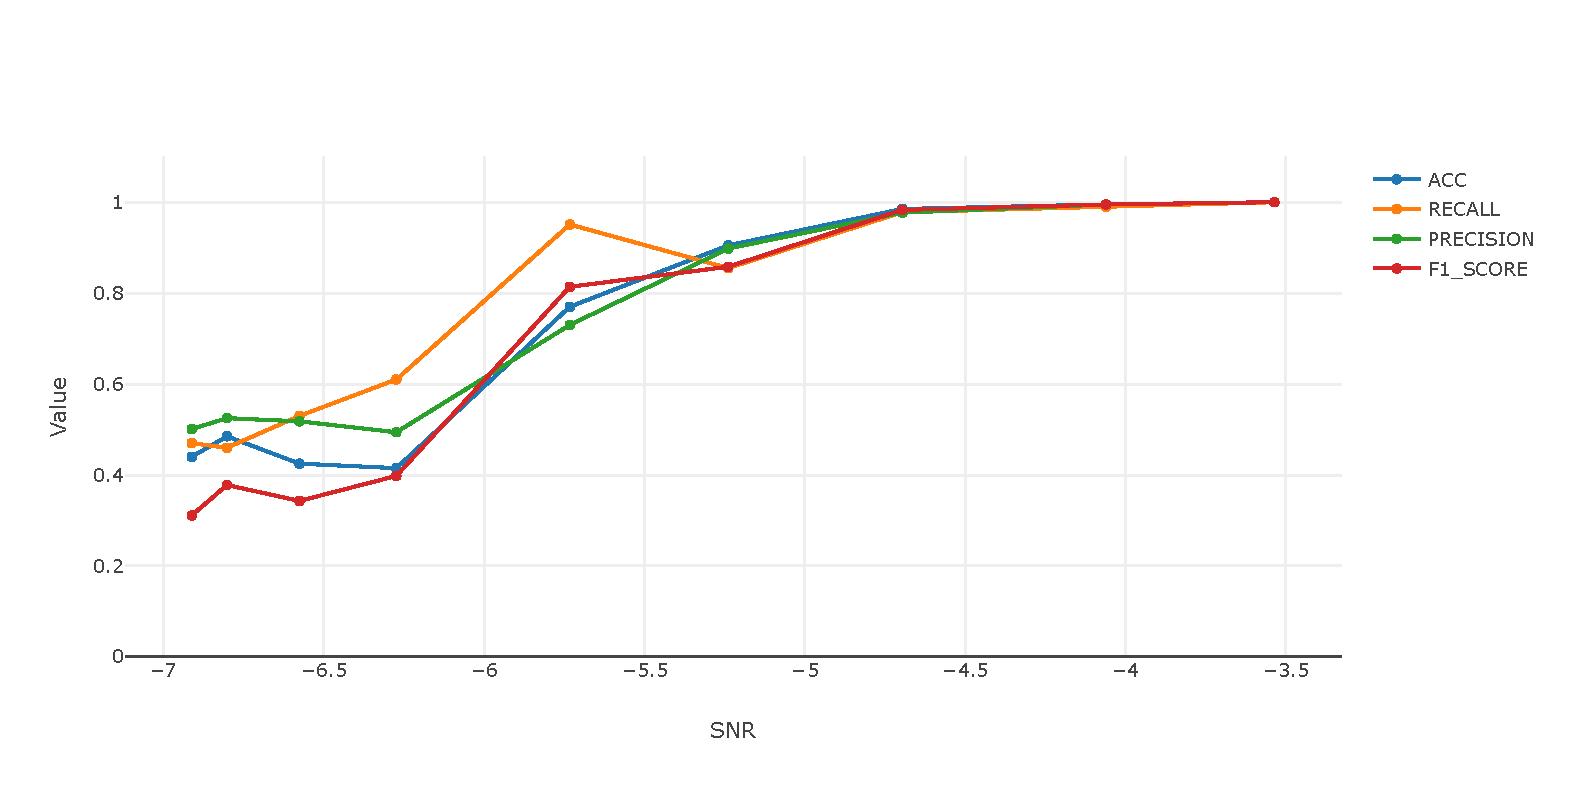
\includegraphics[width=14cm]{images/nn_small_532.pdf}
		\caption{Wyniki dla estymatorów, architektura -5-3-2-}
	\end{figure}

	Zastosowanie surowego sygnału, niezależnie od architektury, daje bardzo chaotyczne wyniki sugerujące że proces nauczania nie przebiega prawidłowo a predykcja jest obarczona dużym błędem. Podejście z zastosowaniem surowego sygnału jest kosztowne obliczeniowo i mało efektywne dlatego należy je wykluczyć z dalszych rozważań. Z kolei zastosowanie estymatorów opisujących sygnał daje obiecujące wyniki pozwalające wnioskować o skutecznym uczeniu się sieci. W oparciu o zaproponowaną architekturę zostanie przeprowadzony kolejny eksperyment mający stwierdzić czy przy użyciu obecnych danych uczących można otrzymać lepsze wyniki.
	
	\subsection{Zależność od architektury}
	Po decyzji o użyciu estymatorów jako danych uczących należy przeprowadzić eksperyment mający na celu określenie najlepszej architektury sieci neuronowej. Ponieważ architektura zaproponowana w poprzednim eksperymencie dawała wyniki świadczące o poprawnie przebiegającym procesie uczenia zaproponowano różne jej wariancje. 
		\begin{figure}[H]
		\centering
		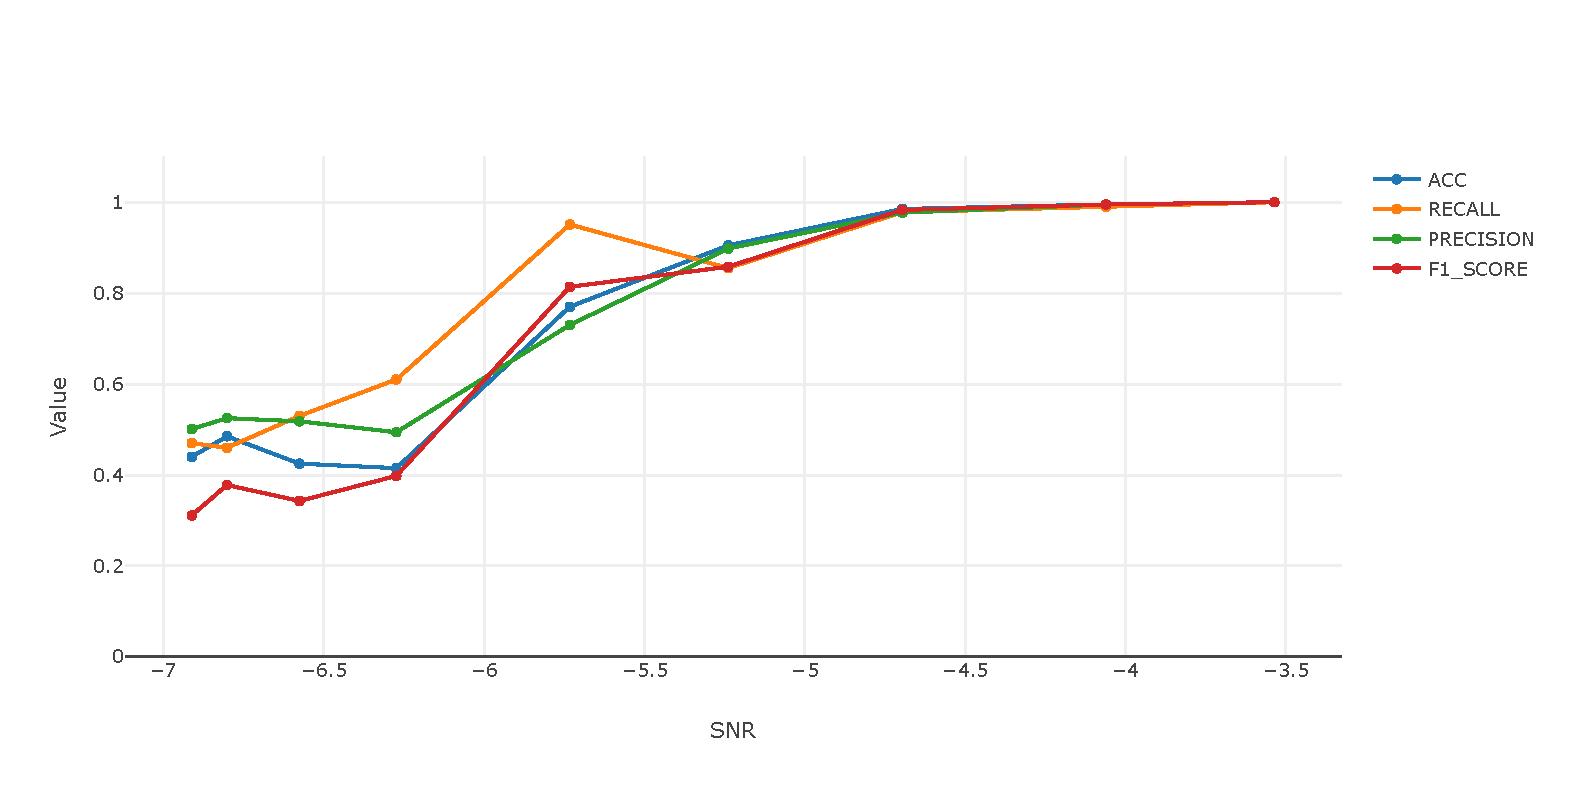
\includegraphics[width=14cm]{images/nn_small_532.pdf}
		\caption{Wyniki dla sieci o architekturze -5-3-2-}
	\end{figure}
	\begin{figure}[H]
		\centering
		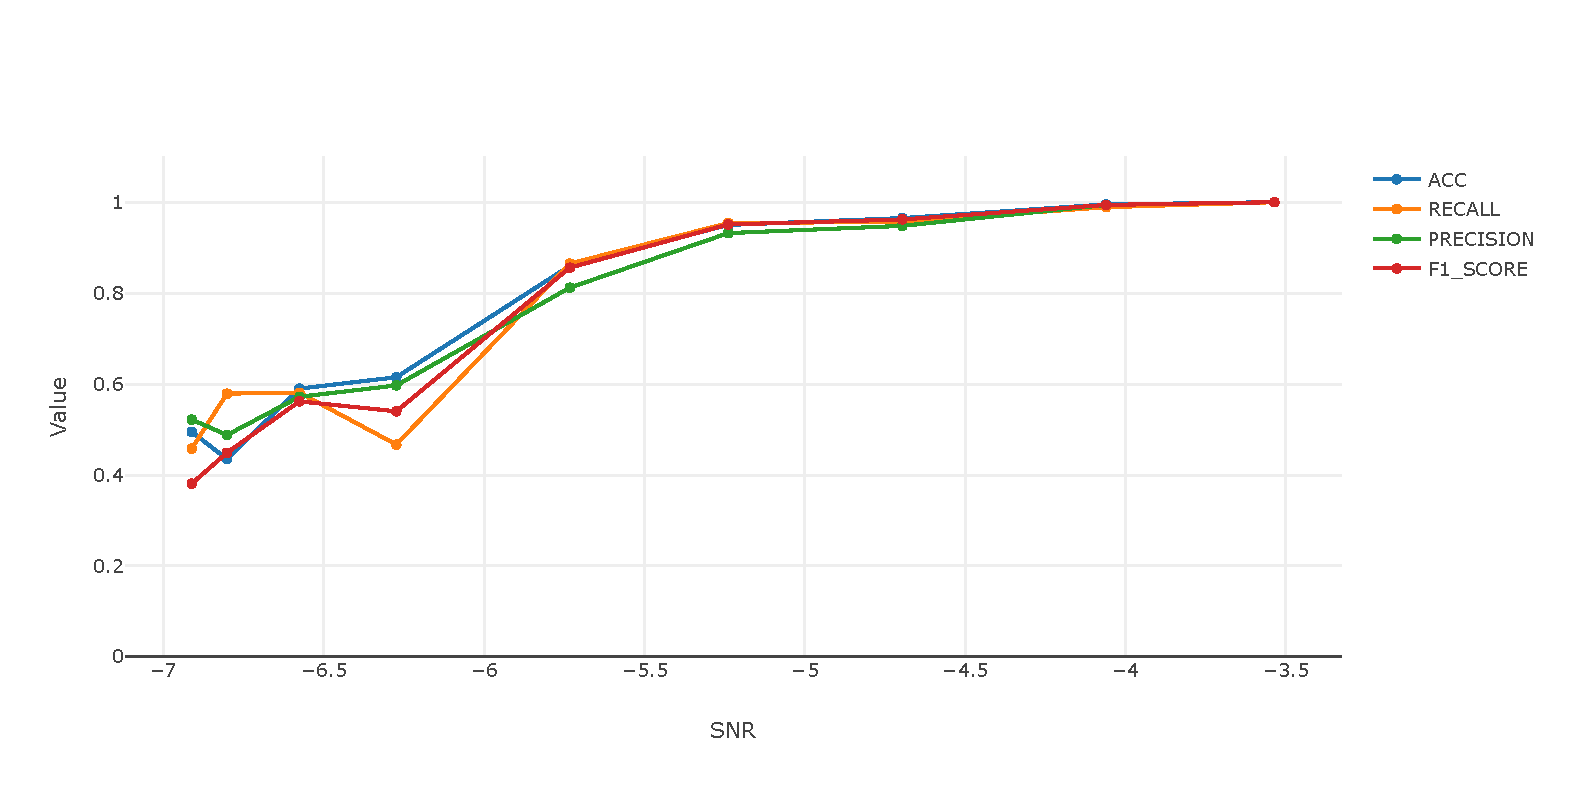
\includegraphics[width=14cm]{images/nn_small_85.pdf}
		\caption{Wyniki dla sieci o architekturze -8-5-}
	\end{figure}
		\begin{figure}[H]
			\centering
			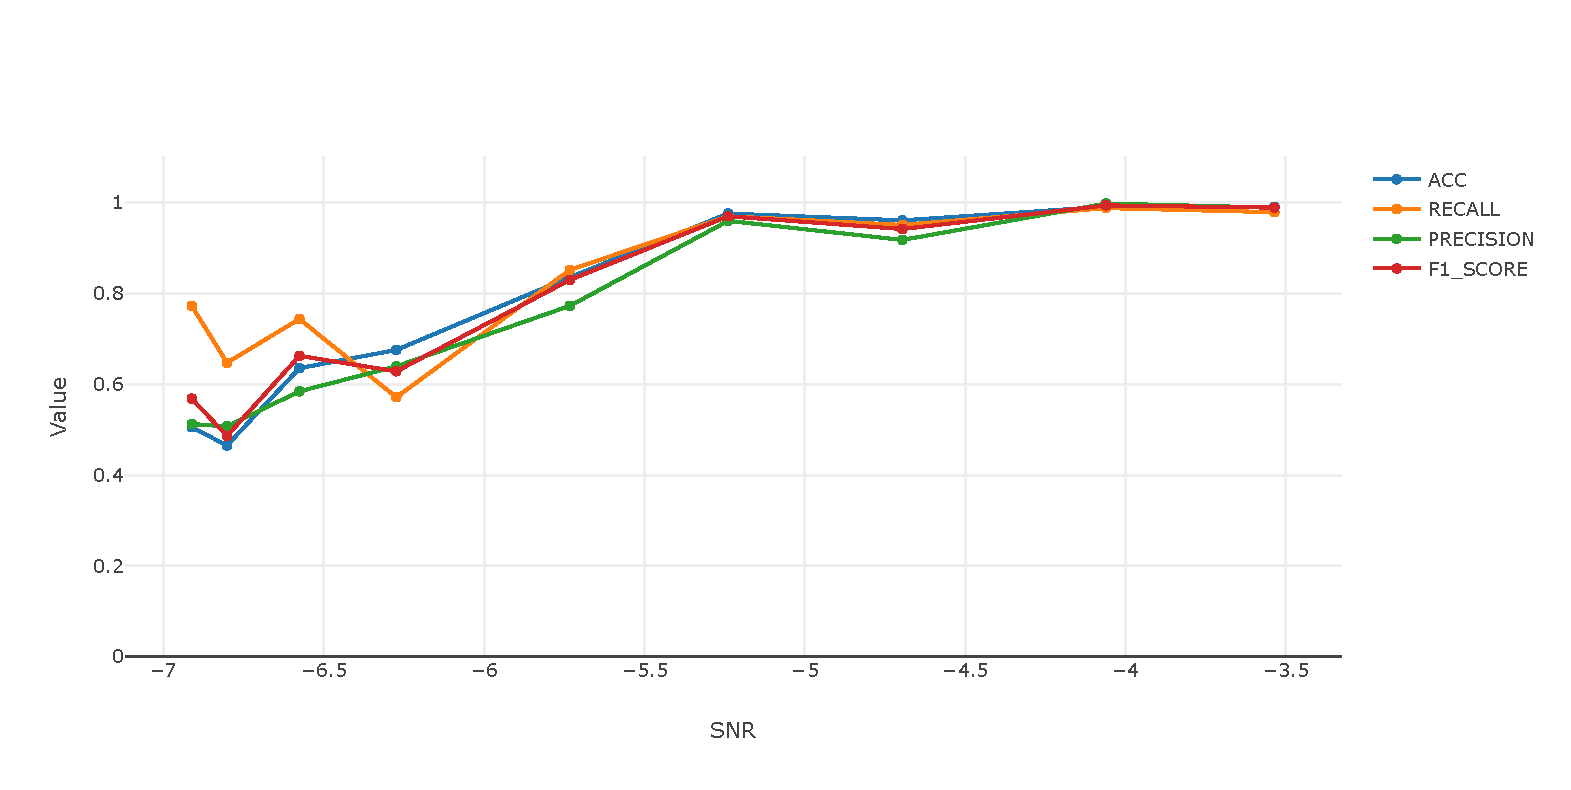
\includegraphics[width=14cm]{images/nn_small_2.pdf}
			\caption{Wyniki dla sieci o architekturze -2-}
		\end{figure}
	\begin{figure}[H]
		\centering
		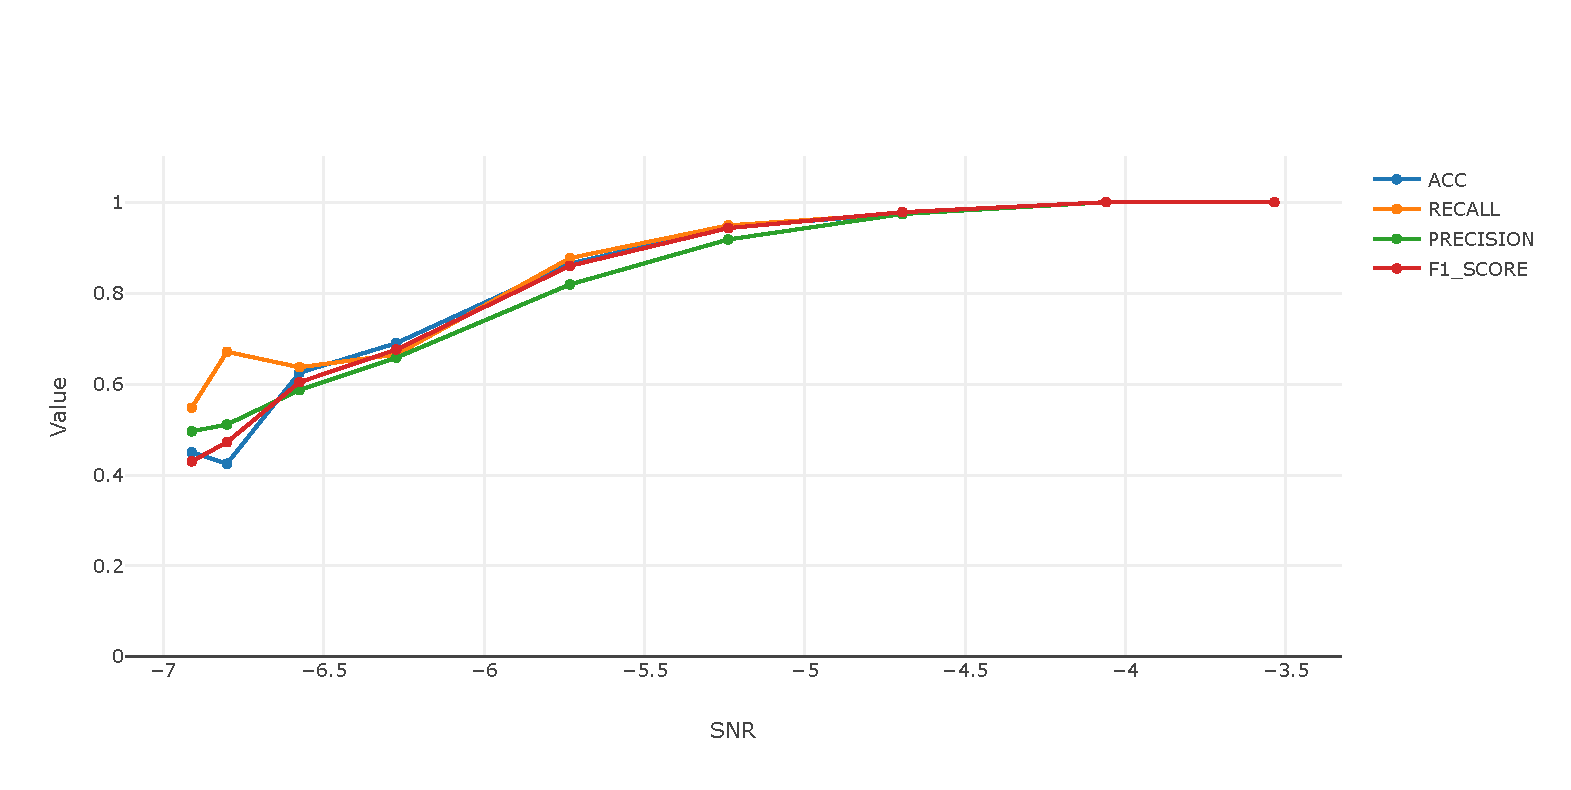
\includegraphics[width=14cm]{images/nn_small_5.pdf}
		\caption{Wyniki dla sieci o architekturze -5-}
	\end{figure}


	
	
	%Nauczanie sieci 
	%Z powodu zapotrzebowania na dużą ilosć danych w procesie uczenia sieci neuronowych dalsza praca opiera się na danych symulowanych. Program generujący sygnał pozwala na dobór szeregu parametrów takich jak częstotliwości, amplitudy, zaszumienie oraz siłę pulsacji.
	%\subsection{Przygotowanie danych}
	%Przed przystąpieniem do uczenia należało przygotować dane uczące, w tym przypadku jest to zestaw sygnałów bez pulsacji oraz sygnałów z różnymi pulsacjami, poniżej przedstawiono tabelkę szczegółowo opisującą przygotowany zbiór danych.
	%\subsection{Surowy sygnał}
	%Pierwszym eksperymentem było przetestowanie jak sieć poradzi sobie w przypadku surowych danych. Do nauczania użyto sygnału odpowiadającemu jednej sekundzie odczytu, co przy próbkowaniu na poziomie $x$ daje $w chuj$ próbek.
	%\\ Tutaj jebniesz schemat sieci
	%\\A tutaj tabelka z wniami 
	%Eksperyment ten przeprowadzony był bardziej dla porównania niż z żeczywistej potrzeby, użycie surowego sygnału i takiej ilości próbek nie wydaje się był optymalnym rozwiązaniem za to jest kosztowne, dobrą praktyką w dziedzinie nauczania maszynowego jest wstępna obróbka danych i znalezienie sposobu na 

	%\subsection{Estymatory}
	
	%\chapter{Wnioski}
	\newpage
	\section{System monitorujący - przykładowe zastosowanie modelu}
	\newpage
	\section{Wnioski}
	\newpage
	
	
	\bibliographystyle{unsrt}
	\bibliography{mybib}
\end{document}